% !TeX program = xelatex
%==============================================================
%  Python金融数据分析 · 第6章 金融时间序列
%  基于《Python金融大数据分析（第2版）》第8章内容改编
%  授课对象：本科金融系学生（已学完第2-5章）
%  编译：xelatex chapter6.tex（编译两遍）
%==============================================================
\documentclass[9pt]{ctexbeamer}

%%%%-----导入宏包-----%%%%
\usepackage{style/shubeamer}   % SHU 主题（配色、帧标题、页脚、Python代码样式）
\usepackage{amsmath,amsfonts,amssymb,bm}
\usepackage{graphicx,hyperref,url}
\usepackage{subcaption}
\usepackage{booktabs}
\usepackage[super,square]{natbib}
\usepackage{wrapfig}          % 文字绕排
\usepackage{calligra}         % 结尾页花体字

%%%%-----设置字体-----%%%%
\setmainfont{CMU Serif}
\setsansfont{CMU Sans Serif}

%%%%-----常用自定义颜色（正文可直接使用）-----%%%%
\definecolor{nvidia}{RGB}{102,156,28}
\definecolor{red}{RGB}{184,13,73}
\definecolor{orange}{RGB}{242,151,36}
\definecolor{darkteal}{RGB}{43,106,108}
\definecolor{darkblue}{RGB}{4,37,58}

%%%%-----每节开始时自动显示当前节目录-----%%%%
\AtBeginSection[]
{
	\begin{frame}<beamer>
		\frametitle{\textbf{目录}}
		\textbf{\tableofcontents[currentsection]}
	\end{frame}
}

%%%%-----设定图片存放路径-----%%%%
\graphicspath{{figures/}}

%%%%-----首页信息设置-----%%%%
\AtBeginDocument{%
	%%%%----短标题[显示在页脚]{封面标题}
	\title[Python金融数据分析 · 第6章]{\fontsize{16pt}{22pt}\selectfont {Python金融数据分析}}
	%%%%----副标题（本章主题）
	\subtitle{\fontsize{9pt}{14pt}\selectfont \textit{第6章\quad 金融时间序列}}
	%%%%----个人信息
	\author[王伟冠]{%
		\begin{tabular}{ll}%
			主讲人： & 王伟冠\tabularnewline%
			院\quad 系： & 经济学院金融系\tabularnewline
		\end{tabular}
	}
	%%%%----机构信息
	\institute[SHU]{上海大学}
	%%%%----日期信息
	\date[\today]{\today}}

%%%%-----数学宏（向量、矩阵、算子等，见 style/macros.tex）-----%%%%
\input{style/macros.tex}


\begin{document}

%% 封面
\begin{frame}
	\titlepage
\end{frame}

%% 目录页
\section*{目录}
\begin{frame}
	\frametitle{\textbf{目录}}
	\textbf{\tableofcontents}
\end{frame}


%==============================================================
\section{真实数据登场}
%==============================================================

\begin{frame}{本章学习目标}
	\begin{itemize}
		\item 首次使用\textbf{真实市场数据}：2010--2018年美股、指数、外汇、黄金
		\item 掌握收益率的两种算法：简单收益率与对数收益率，及其适用场景
		\item 会用滚动窗口计算移动平均与滚动波动率，观察\alert{波动率聚集}
		\item 理解收益率分布的\alert{厚尾}现象及其风险管理含义
		\item 会用 OLS 回归估计股票的 beta，理解相关与回归的区别
	\end{itemize}
	\begin{block}{本章数据}
		教材配套数据集 \texttt{eod\_data.csv}（来源：Refinitiv Eikon），12 个资产的日频收盘价。
	\end{block}
\end{frame}

\begin{frame}[fragile]{读入真实数据}
	\begin{lstlisting}
import numpy as np
import pandas as pd

df = pd.read_csv("../data/eod_data.csv",    # 本章data目录
                 index_col=0,       # 第0列(日期)作索引
                 parse_dates=True)  # 解析成日期类型
df.shape          # (2216, 12)：8年半，2216个日期
df.columns.tolist()
\end{lstlisting}
	\begin{lstlisting}
['AAPL.O', 'MSFT.O', 'INTC.O', 'AMZN.O', 'GS.N', 'SPY',
 '.SPX', '.VIX', 'EUR=', 'XAU=', 'GDX', 'GLD']
\end{lstlisting}
	\begin{itemize}
		\item 个股（苹果、微软\ldots）、标普500指数 \texttt{.SPX}、波动率指数 \texttt{.VIX}、
			欧元汇率 \texttt{EUR=}、黄金 \texttt{XAU=} 等。
		\item 不同市场的交易日不完全重合，所以表里有 \texttt{NaN}——真实数据的常态。
	\end{itemize}
\end{frame}

\begin{frame}[fragile]{数据体检：缺失值在哪里？}
	\begin{lstlisting}
df.isna().sum()      # 每列缺失个数
df = df.dropna(subset=["SPY", "AAPL.O"])  # 只保留美股交易日
df.shape             # (2138, 12)
\end{lstlisting}
	\begin{itemize}
		\item 以 SPY（美股ETF）为准过滤日期：只研究美股交易日。
		\item 其他资产（黄金、外汇）在美股假日缺失的部分仍保留为 \texttt{NaN}，
			后续用到时再单独处理。
	\end{itemize}
	\begin{alertblock}{零基础提醒}
		\texttt{NaN} 参与任何运算结果都是 \texttt{NaN}；
		统计函数（\texttt{mean/std}）会自动跳过它——但要知道它存在。
	\end{alertblock}
\end{frame}

\begin{frame}{先看全景：归一化价格}
	\begin{figure}
		\centering
		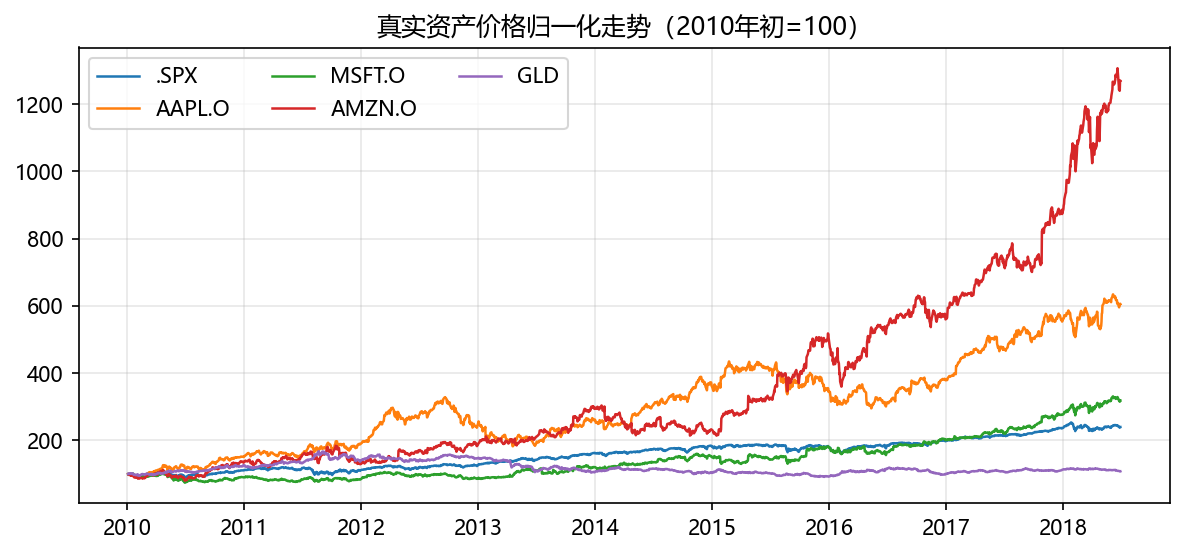
\includegraphics[width=0.88\textwidth]{fts_norm_prices}
		\caption{各资产以2010年初为100归一化——苹果、微软、亚马逊八年间的巨大涨幅一目了然}
	\end{figure}
\end{frame}

\begin{frame}[fragile]{归一化的代码}
	\begin{lstlisting}
sel = [".SPX", "AAPL.O", "MSFT.O", "AMZN.O", "GLD"]
norm = df[sel] / df[sel].iloc[0] * 100   # 起点=100
norm.plot(figsize=(8, 4), grid=True)
\end{lstlisting}
	\begin{itemize}
		\item 不同资产价格量级差异大（黄金上千、汇率1.4），直接画没法比。
		\item 除以各自首日价格再乘100：把"价格"变成"涨跌幅指数"。
		\item 向量化除法对整个 DataFrame 生效——第3、4章功力的直接应用。
	\end{itemize}
\end{frame}


%==============================================================
\section{收益率：金融数据的"通用语言"}
%==============================================================

\begin{frame}[fragile]{简单收益率 vs 对数收益率}
	\begin{lstlisting}
simple = df["SPY"].pct_change()          # (今日-昨日)/昨日
logret = np.log(df["SPY"] / df["SPY"].shift(1))
logret.head()
\end{lstlisting}
	\begin{lstlisting}
Date
2010-01-04         NaN
2010-01-05    0.002644
2010-01-06    0.000704
Freq: B, Name: SPY, dtype: float64
\end{lstlisting}
	\begin{itemize}
		\item 对数收益率 $r_t = \ln(P_t / P_{t-1})$；日常涨跌小时，两者数值几乎相同。
		\item 对数收益率的优点：\alert{可以直接加总}——日收益相加即区间收益。
	\end{itemize}
	\begin{alertblock}{为什么要取对数？}
		$\ln(P_T/P_0) = \ln(P_T/P_{T-1}) + \cdots + \ln(P_1/P_0)$，
		简单收益率连乘才等价，统计建模中加法形式友好得多。
	\end{alertblock}
\end{frame}

\begin{frame}[fragile]{一张表算出所有资产的收益率}
	\begin{lstlisting}
rets = np.log(df / df.shift(1))   # 12列一次全算
rets.describe().round(4)          # 每列的统计摘要
\end{lstlisting}
	\begin{itemize}
		\item \texttt{df / df.shift(1)}：整表除以"昨天的自己"。
		\item 第一行全是 \texttt{NaN}（没有"昨天"）——\texttt{dropna()} 或让函数自动跳过。
		\item 观察 \texttt{describe()}：均值接近0、标准差差异大（VIX 日波动最大）。
	\end{itemize}
	\begin{block}{年化：从日到年}
		年化均值 $\approx$ 日均值 $\times 252$；
		年化波动率 $=$ 日波动率 $\times \sqrt{252}$。\\
		252 是一年的交易日数，金融计算的常用常数。
	\end{block}
\end{frame}

\begin{frame}[fragile]{年化统计量}
	\begin{lstlisting}
rets.mean() * 252                # 年化平均收益
rets.std() * np.sqrt(252)        # 年化波动率
(rets["AAPL.O"] * 252).round(3)  # 苹果：约0.21（21%）
\end{lstlisting}
	\begin{itemize}
		\item 为什么波动率乘 $\sqrt{252}$ 而不是 252？方差按时间线性累加，
			标准差（波动率）按平方根累加。
		\item 比较不同资产的风险收益，必须放在同一时间尺度上——年化是行业标准。
	\end{itemize}
\end{frame}

\begin{frame}[fragile]{重采样：日频 $\to$ 月频/年频}
	\begin{lstlisting}
df.resample("ME").last()     # 每月最后一个交易日的价格
df.resample("YE").last()     # 每年最后一个交易日
rets.resample("ME").sum()    # 对数收益按月加总=月收益
\end{lstlisting}
	\begin{itemize}
		\item 真实分析常需要换频率：月报、年度回顾、周度策略。
		\item 价格取 \texttt{last}，对数收益取 \texttt{sum}——语义不同，别混用。
	\end{itemize}
\end{frame}


%==============================================================
\section{滚动统计与波动率聚集}
%==============================================================

\begin{frame}[fragile]{rolling：移动窗口}
	\begin{lstlisting}
spy = rets["SPY"].dropna()
ma21  = spy.rolling(21).mean()   # 21日移动平均
vol21 = spy.rolling(21).std() * np.sqrt(252)  # 滚动年化波动率
vol21.head(25)    # 前20个是NaN：窗口不足
\end{lstlisting}
	\begin{itemize}
		\item \texttt{rolling(n)}：每次取最近 $n$ 个数据算统计量，窗口逐日滑动。
		\item 前 $n-1$ 个结果为 \texttt{NaN}——数据不足，正常现象。
		\item 技术分析中的 MA5、MA20、MA60 就是不同窗口的移动平均。
	\end{itemize}
\end{frame}

\begin{frame}{波动率聚集：大波动跟着大波动}
	\begin{figure}
		\centering
		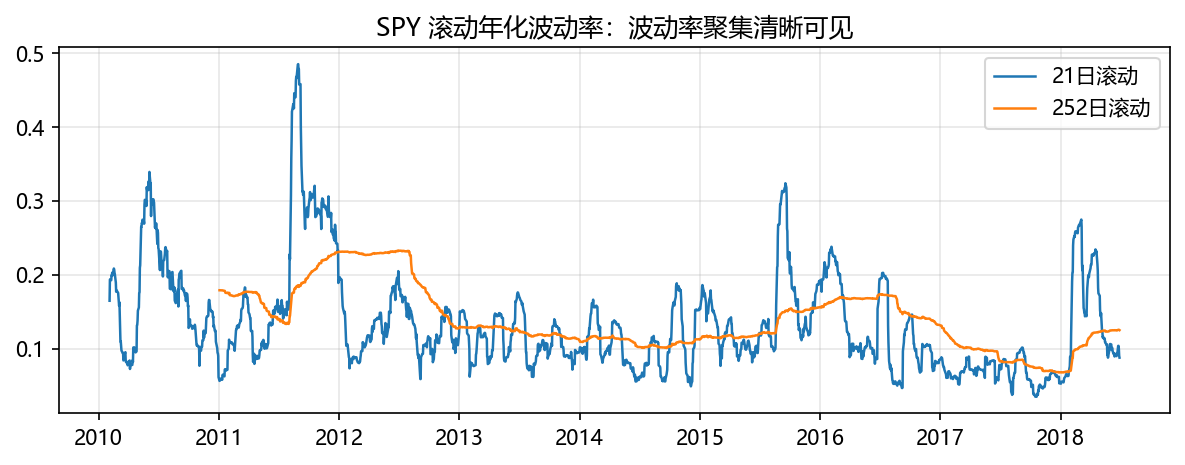
\includegraphics[width=0.9\textwidth]{fts_roll_vol}
		\caption{SPY 滚动年化波动率：2011年欧债危机、2015年人民币汇改与2018年初的波动尖峰}
	\end{figure}
\end{frame}

\begin{frame}{波动率聚集的要点}
	\begin{itemize}
		\item 波动率不是平稳的：平时低，危机时突然飙升，然后缓慢回落。
		\item 这个现象叫\textbf{波动率聚集}（volatility clustering），
			是金融时间序列最著名的"程式化事实"之一。
		\item 实际意义：
		\begin{itemize}
			\item 风险度量（VaR）必须用\alert{最近}的数据，而不是八年平均；
			\item 21日窗口反应快但噪声大，252日窗口平滑但迟钝——窗口选择是权衡。
		\end{itemize}
	\end{itemize}
	\begin{alertblock}{不要犯的错}
		用全样本的标准差代表"日常风险"——会严重低估危机时期的损失。
	\end{alertblock}
\end{frame}


%==============================================================
\section{收益率分布与厚尾}
%==============================================================

\begin{frame}{SPY 日收益率分布}
	\begin{figure}
		\centering
		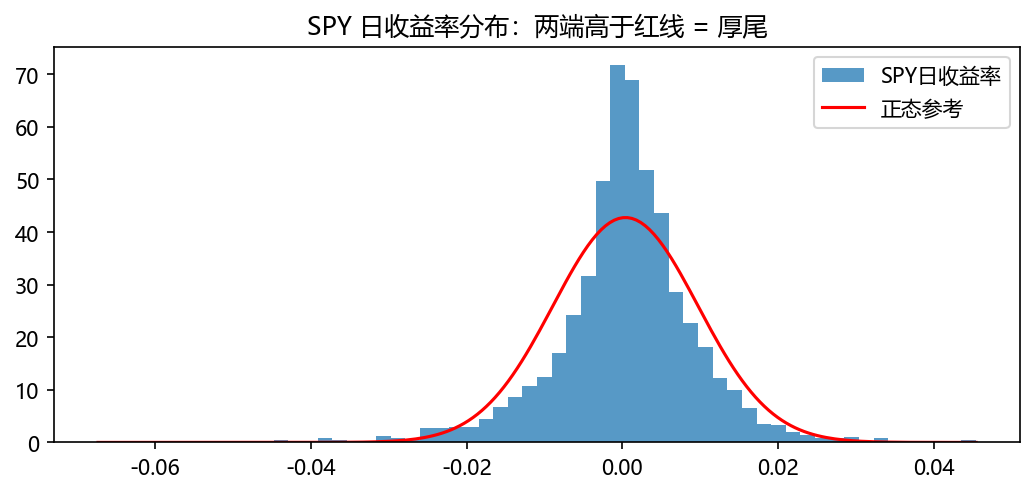
\includegraphics[width=0.8\textwidth]{fts_hist}
		\caption{直方图与正态分布（红线）对比：两端的柱子明显高于红线}
	\end{figure}
\end{frame}

\begin{frame}[fragile]{厚尾的定量证据}
	\begin{lstlisting}
r = rets["SPY"].dropna()
(r.abs() > 0.03).sum()    # |日收益|>3%的天数
\end{lstlisting}
	\begin{lstlisting}
27
\end{lstlisting}
	\begin{itemize}
		\item 8年半约 2137 个交易日，按正态分布（日标准差约1\%）计算，
			$|r|>3\%$ 几乎不可能发生（理论上不到 1 天），实际却有 \alert{27 天}。
		\item 单日涨跌超 3\% 在正态下是"万年一遇"，现实中平均每三个月就出现一次。
	\end{itemize}
	\begin{alertblock}{风险管理核心教训}
		\textbf{厚尾}：极端行情远比正态分布预想的频繁。
		模型假设正态，会系统性低估尾部风险。
	\end{alertblock}
\end{frame}


%==============================================================
\section{回归分析：beta是怎么算出来的}
%==============================================================

\begin{frame}[fragile]{CAPM 与 beta}
	\begin{itemize}
		\item 资本资产定价模型（CAPM）：个股收益与市场收益线性相关
	\end{itemize}
	\begin{equation*}
		r_i = \alpha + \beta \, r_m + \varepsilon
	\end{equation*}
	\begin{itemize}
		\item $\beta$：股票对市场波动的敏感度。$\beta=1$ 与市场同步；
			$\beta>1$ 放大波动；$\beta<1$ 相对稳健。
		\item 估计方法：把历史日收益做\textbf{最小二乘回归}（OLS）。
	\end{itemize}
	\begin{lstlisting}
x = rets[".SPX"].dropna()      # 市场收益
y = rets["AAPL.O"].dropna()    # 苹果收益
beta, alpha = np.polyfit(x, y, 1)   # 一元线性拟合
round(beta, 2)
\end{lstlisting}
\end{frame}

\begin{frame}{回归结果可视化}
	\begin{figure}
		\centering
		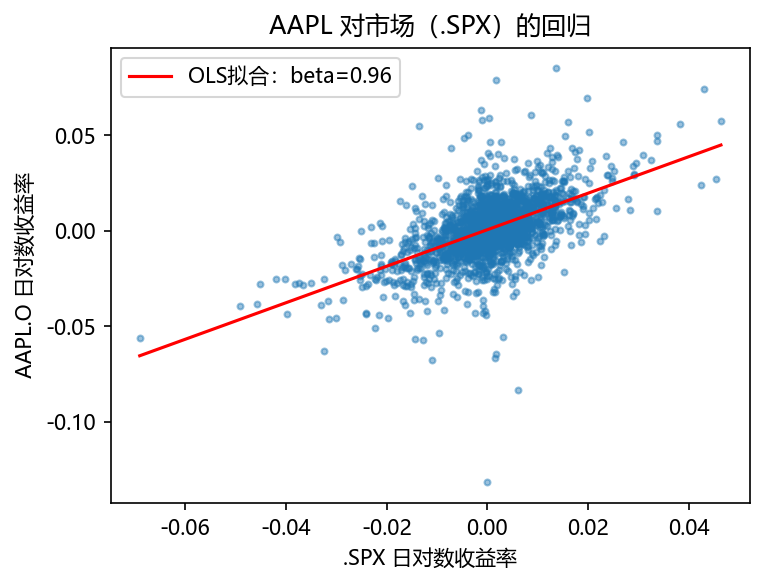
\includegraphics[width=0.62\textwidth]{fts_regression}
		\caption{AAPL 对 .SPX 日收益回归：beta $\approx$ 0.96，接近市场平均水平}
	\end{figure}
\end{frame}

\begin{frame}[fragile]{相关系数 vs 回归系数}
	\begin{lstlisting}
x.corr(y)    # 相关系数：约0.57
\end{lstlisting}
	\begin{itemize}
		\item \textbf{相关系数}衡量"联动紧密程度"，范围 $[-1, 1]$；
		\item \textbf{beta} 衡量"市场涨1\%，个股平均涨多少"，可以大于1或为负。
		\item 两者关系：$\beta = \rho \cdot \sigma_i / \sigma_m$。
	\end{itemize}
	\begin{exampleblock}{换个视角：VIX 恐慌指数}
		\texttt{df[".VIX"].corr(日收益)} 为负（约 $-0.18$）：市场恐慌升高时，股价倾向下跌。
		VIX 常被称为"恐慌指数"。
	\end{exampleblock}
\end{frame}

\begin{frame}{VIX 与市场收益的负相关}
	\begin{figure}
		\centering
		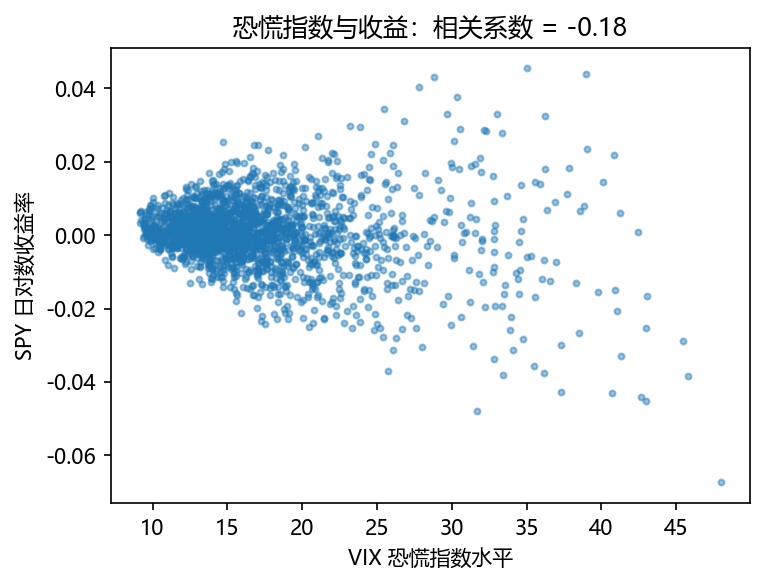
\includegraphics[width=0.6\textwidth]{fts_vix}
		\caption{VIX 越高（横轴右侧），SPY 日收益越倾向为负}
	\end{figure}
\end{frame}


%==============================================================
\section{小结与练习}
%==============================================================

\begin{frame}{本章小结}
	\begin{itemize}
		\item \textbf{真实数据}：\texttt{read\_csv} + 缺失值处理（\texttt{dropna}）是第一步。
		\item \textbf{收益率}：对数收益率可加性好，是建模首选；
			年化规则：均值 $\times 252$，波动率 $\times \sqrt{252}$。
		\item \textbf{滚动窗口}：\texttt{rolling(n).mean()/std()}——
			移动平均与滚动波动率；波动率聚集要求风险度量用近期数据。
		\item \textbf{厚尾}：极端行情比正态假设更常见，风险管理不能只靠均值方差。
		\item \textbf{回归}：\texttt{np.polyfit} 一行估计 beta；
			相关系数说联动程度，beta 说敏感度。
	\end{itemize}
\end{frame}

\begin{frame}{课后任务与下章预告}
	\begin{block}{课后任务}
		\begin{enumerate}
			\item 对 MSFT.O 重复 beta 回归，比较与苹果的 beta 大小，
				并结合两家公司的业务特点给出解释。
			\item 把滚动波动率窗口从 21 改为 63（一个季度），
				观察图形平滑程度的变化。
			\item 选做：统计 $|r|>5\%$ 的天数，查一查这些日期分别对应什么历史事件，
				进一步体会厚尾。
		\end{enumerate}
	\end{block}
	\begin{exampleblock}{下章预告}
		数据从哪来？下一章讲 \textbf{数据输入输出}：CSV、Excel、HDF5，
		以及更大规模数据的存取方式。
	\end{exampleblock}
	\begin{center}
		\vspace{0.5em}
		本章内容改编自教材第8章\citep{hilpisch2018python}。
	\end{center}
\end{frame}


%==============================================================
%  附录：参考文献 + 结尾页
%==============================================================
\appendix

\begin{frame}[allowframebreaks]{参考文献}
	\bibliographystyle{style/gbt7714-2005}
	\bibliography{reference.bib}
\end{frame}

\begin{frame}
	\begin{center}
		{\Huge\calligra Thanks for your attention!}
		\vspace{1cm}

		{\Huge Q \& A}
	\end{center}
\end{frame}

\end{document}
